\documentclass[10pt,a4paper]{book}
\usepackage{graphicx}
\graphicspath{{figures/}}

\title{A Laboratory Course on Single Molecule Localization Microscopy}

\author{Kyle M. Douglass}

\date{\today}

\begin{document}

\maketitle

\chapter{Introduction}

\section{Superresolution Fluorescence Microscopy}

Fluorescence microscopy is a set of techniques that allows scientists to study the structure and behavior of microscopic systems. Cell biologists in particular use fluorescence microscopes to visualize biological systems across many different spatial scales, from macromolecular complexes, organelles, and cells to tissues and even whole organisms. The power of fluorescence microscopy comes from the ability to label specific molecules with fluorescent markers such that the presence of light coincides with the presence of the target molecules. This molecular specificity, when combined with a light microscope's ability to magnify specimens that are normally too small to see with the unaided eye, provides a powerful tool to better understand the microscopic world.

All light microscopes, however, are bound by the laws of diffraction which state that the smallest features that can be observed by the instrument are approximately the size of the wavelength of light. Anything smaller than this so-called diffraction limit appears blurred, often to the point where an observer is completely unable to infer its structure from an image. For biologists this is particularly problematic because many important cellular structures have sizes that are smaller than this limit.

\section{Learning Outcomes}

\begin{enumerate}
    \item Explain how a modern epifluorescence microscope works, including a list of its main components and their relationships to one another.
    \item Identify the main components of an epifluorescence microscope on the real microscope in the lab.
    \item Explain the principle behind single molecule localization microscopy and how it overcomes the diffraction limit of light.
    \item Model fluorescence phenomena such as photoswitching and photoactivation as continuous-time Markov chains.
    \item Analyze data from the microscope to produce super-resolved images of cellular structures.
\end{enumerate}

\chapter{The Modern Fluorescence Microscope}

\chapter{Single Molecule Localization Microscopy}

\chapter{Fluorescence Photophysics}

\chapter{Localization Microscopy in Practice}

\begin{figure}[ht]
    \centering
    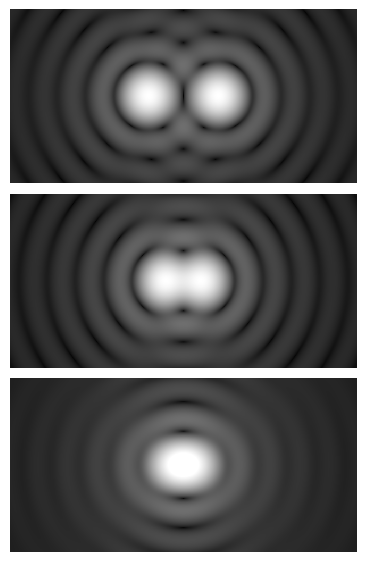
\includegraphics[width=0.75\textwidth]{Airy_disk_spacing_near_Rayleigh_criterion.png}
    \caption{Rayleigh criterion}
    \label{fig:rayleigh}
\end{figure}

\end{document}
